\documentclass[pdf]{beamer}
\mode<presentation>{}
\usetheme{Dresden}
\usepackage{apalike}
\usepackage{graphicx}
\usepackage{subcaption}
\usepackage{pgfplotstable}
\usepackage{graphicx,psfrag}
\usepackage{mwe,tikz}\usepackage[percent]{overpic}
%% preamble
\title{Robust Computational Models for Water Waves}
\author{Jordan Pitt, Stephen Roberts and Christopher Zoppou \\ Australian National University}
\newcommand\solidrule[1][0.25cm]{\rule[0.5ex]{#1}{1pt}}
\newcommand\dashedrule{\mbox{\solidrule[2mm]\hspace{2mm}\solidrule[2mm]}}
\newcommand{\dotrule}[1]{%
	\parbox[]{#1}{\dotfill}}

\begin{document}
%% title frame
\section{Introduction}
\begin{frame}
\titlepage
\end{frame}
\begin{frame}{Outline of the Presentation}
	\begin{itemize}
		\item Water Wave Modelling
		\item Robust Computational Models
	\end{itemize}
\end{frame}

\section{Water Wave Modelling}
\begin{frame}{Modelling}
	%Picture Physical Process -> Mathematical Description -> Studying Mathematical Description (Numerical Solution)
	\begin{figure}
		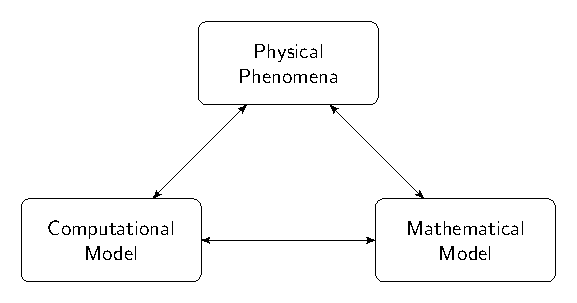
\includegraphics[width=\textwidth]{./Pics/ModelDiagrams/FlowChart.pdf}
	\end{figure}
\end{frame}
\begin{frame}{Physical Phenomena}
	%Picture Physical Process -> Mathematical Description -> Studying Mathematical Description (Numerical Solution)
	\begin{figure}
		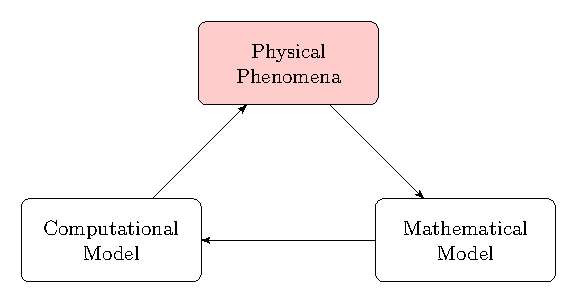
\includegraphics[width=\textwidth]{./Pics/ModelDiagrams/FlowChartHigh1.pdf}
	\end{figure}
\end{frame}
\begin{frame}{Physical Phenomena: Water Waves}
	Water wave hazards:
		\begin{itemize}
			\item Tsunamis
			\item Storm Surges
			\item Rogue Waves
		\end{itemize}
	\smallskip
	Phenomena caused by water waves:
		\begin{itemize}
			\item Nutrient Transport
			\item Beach Erosion
			\item Breakup of Sea Ice
		\end{itemize}
\end{frame}
%Cool pictures
\begin{frame}{Typical Scenario}
	\begin{figure}
		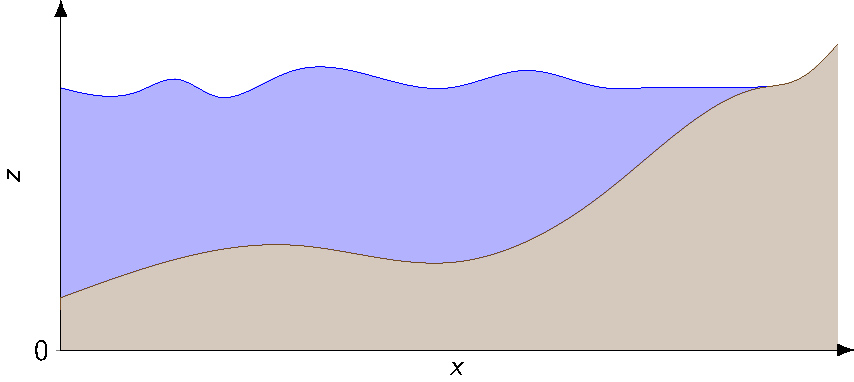
\includegraphics[width=\textwidth]{./Pics/WaterModelDiagrams/FressSurface.pdf}
	\end{figure}
\end{frame}


\subsection{Free Surface Flows}
\begin{frame}{Mathematical Model}
	%Picture Physical Process -> Mathematical Description -> Studying Mathematical Description (Numerical Solution)
	\begin{figure}
		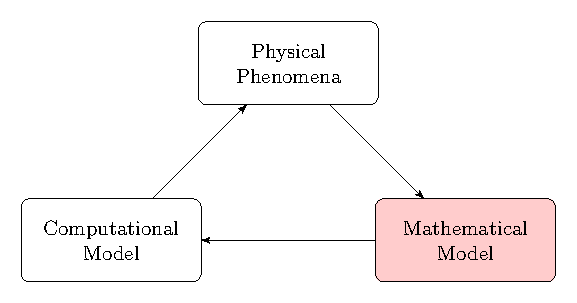
\includegraphics[width=\textwidth]{./Pics/ModelDiagrams/FlowChartHigh2.pdf}
	\end{figure}
\end{frame}
\begin{frame}{Navier Stokes Model}
	\begin{figure}
		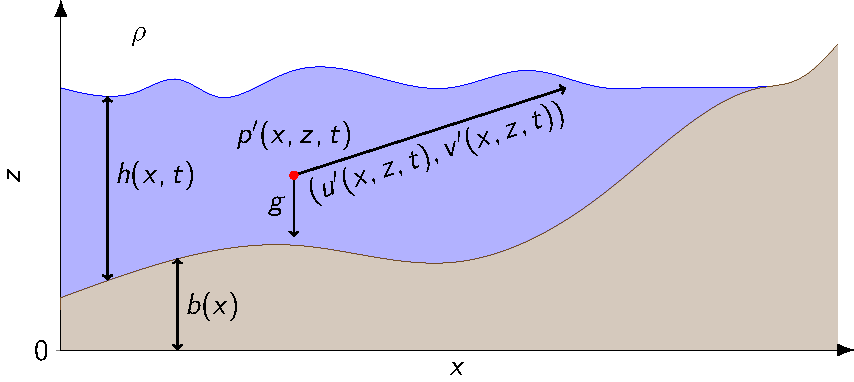
\includegraphics[width=\textwidth]{./Pics/WaterModelDiagrams/NavierStokes.pdf}
	\end{figure}
\end{frame}
\begin{frame}{Pros and Cons}
\end{frame}

\subsection{Shallow Water Wave Model}
\begin{frame}{Shallow Water Wave Model}
	\begin{figure}
		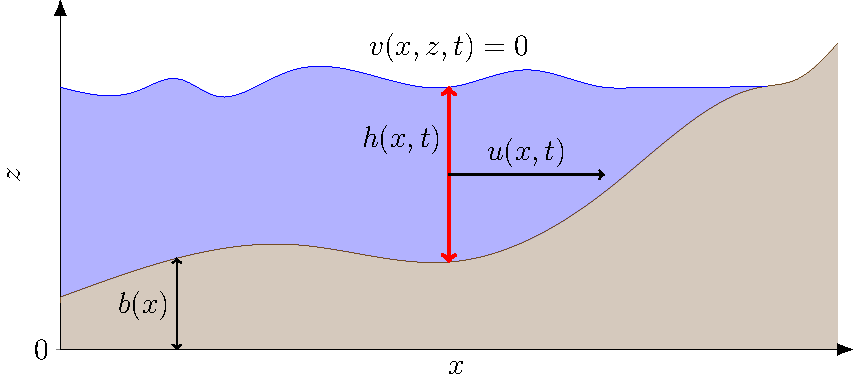
\includegraphics[width=\textwidth]{./Pics/WaterModelDiagrams/SWWE.pdf}
	\end{figure}
\end{frame}
\begin{frame}{Pros and Cons}
\end{frame}
\begin{frame}{Previous Work}
\end{frame}
%mention previous work of ANU


\subsection{Serre Model}

\begin{frame}{Serre Model}
	\begin{figure}
		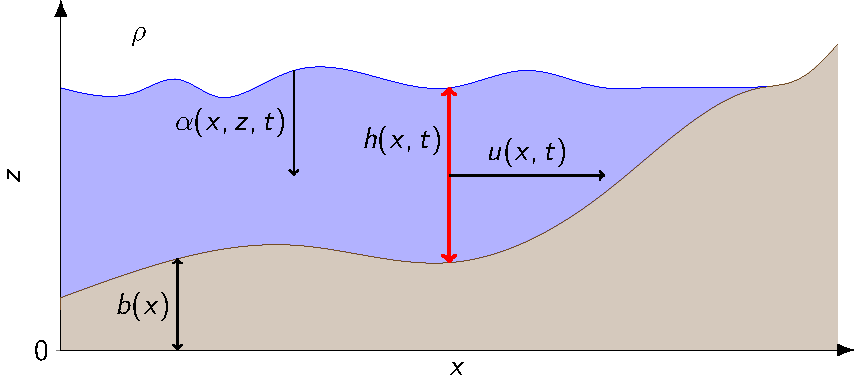
\includegraphics[width=\textwidth]{./Pics/WaterModelDiagrams/Serre.pdf}
	\end{figure}
\end{frame}
\begin{frame}{Pros and Cons}
\end{frame}
\begin{frame}{Previous Work}
\end{frame}


\section{Robust Computational Model}
%Goal of thesis to develop numerical method that can handle dry beds and steep gradients using FEM and FVM

\begin{frame}{Computational Model}
	\begin{figure}
		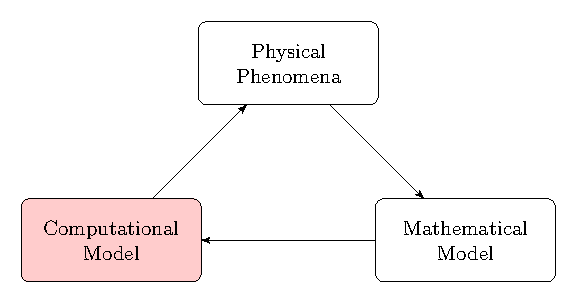
\includegraphics[width=\textwidth]{./Pics/ModelDiagrams/FlowChartHigh3.pdf}
	\end{figure}
\end{frame}
\subsection{Steep Gradients in the Flow}
%What was known
%Previous Work
%Improvements
\begin{frame}
\end{frame}
\subsection{Dry Beds}
%What was known
%Previous Work
%Improvements
\begin{frame}
\end{frame}

\end{document}